\part{Seminar 7 - Winding Configurations and Optimal Stator and Rotor Pole Combination of Flux-Switching PM Brushless AC Machines}

\makebox[.25\textwidth]{John Moraine}\makebox[.25\textwidth]{Thomas Desbrosses}\makebox[.25\textwidth]{Thomas Collette}\makebox[.25\textwidth]{Eleonore Masarweh}

\section{Introduction and reminders}
The presentation was based on two distinct articles both detailing the flux switching permanent magnet (FSPM) machines. The first article : \textit{"Comparison of All- and Alternate-Poles-Wound FSPM Machines Having Different Stator and Rotor Pole Numbers"} analyzes and compares results of FSPM machines with different rotor/stator combinations. It is a purely data oriented article that has, on it's own, little to no purpose. On the other hand, the second article : \textit{"Winding Configurations and Optimal Stator and Rotor Pole Combination of Flux-Switching PM Brushless AC Machines"} is much more interesting. It develops the FSPM machine : it's structure, operating principle and the different parameters that are studied in order to optimise its use. It is the latter article that is important to understand; the former can be interesting to browse to observe the influence of different stator/rotor couples on the crucial parameters.

%

\section{Structure of the machine and operating principle}
\subsection{Topology}
The machine is made of : 
\begin{itemize}
    \item a stator with teeth made of 
        \begin{itemize}
            \item Permanent magnets aligned with the $e_\theta$ direction
            \item U shaped iron parts
        \end{itemize}
    \item a solid iron rotor (solid means here that it is only one piece) 
\end{itemize}
All of this can be seen in Figure \ref{fig:FSPMTop}. 
\begin{figure}
    \centering
    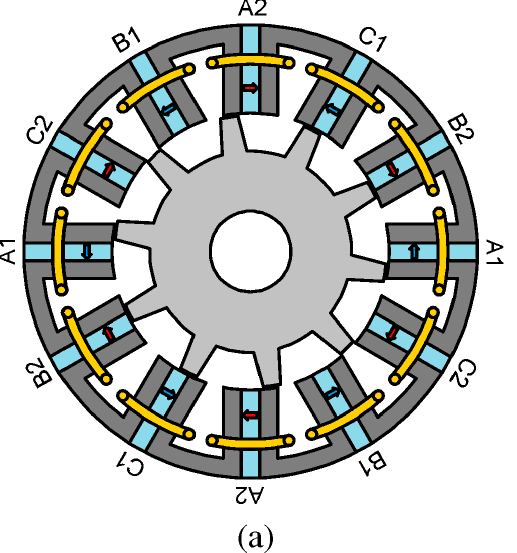
\includegraphics[width=0.5\textwidth]{FSPMTop.png}
    \caption{FSPM machine topology}
    \label{fig:FSPMTop}
\end{figure}

The consequences of such a topology are : a reduced slot area (due to the magnets) and a much easier thermal management of the rotor compared to machines having magnets on the rotor (FSCW, see seminar 6). 

\subsection{Working principle}
Also named 'how the hell does this turn?'. 

\subsubsection{Basic principles}
The rotor in front of the tooth as three main possible configurations : 
\begin{itemize}
    \item maximal flux in positive sense, the rotor tooth is perfectly in front of the first iron part of the tooth, this position is a preferential one
    \item minimal flux (or flux cancellation), the rotor tooth is either in front of the magnet or exactly between two stator teeth
    \item maximal flux in the negative sens, the rotor tooth is in front of the second iron part of the tooth, also a preferential position
\end{itemize}
Intermediate positions also exists but these positions induce a strong torque as the stator-rotor tooth system heads towards a preferential position. This is shown in Figure \ref{fig:fluxswitching}.
\begin{figure}
    \centering
    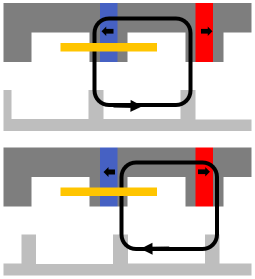
\includegraphics[width=0.4\textwidth]{fluxSwitching.png}
    \caption{Preferential positions of maximal flux}
    \label{fig:fluxswitching}
\end{figure}

\subsubsection{Turning machine}
Given that there are preferential positions, it is evident that the machine will not be able to turn if every stator tooth is in front of a rotor one. To avoid this situation, the FSPM machine never has the same number of stator and rotor poles. The torque is induced by the flux switching in the coils.

\section{Electromagnetic torque}

\subsection{Torque expression}
First we start with the general expression of the torque in an electromechanical converter.
$$ T_{em} ~~ = ~~  \frac{\partial W_{cmag0}(\theta_{m})}{\partial \theta_{m}} ~~+~~ \sum_{k=1}^{n} \frac{\partial \psi_{k0}(\theta_{m})}{\partial \theta_{m}} i_{k} ~~+~~ \frac{1}{2} \sum_{k=1}^{n} \sum_{j=1}^{n} \frac{\partial L_{kj}(\theta_{m})}{\partial \theta_{m}} i_{k}i_{j} $$
The first term is the cogging torque which will be high only if there is a preferential position of the rotor in the stator. It happens only if both have the same number of poles, and as we want to avoid this situation we will consider that their number of poles are chosen to be different. This preferential position is intuitive because if we have $N_{r} = N_{s}$, all the poles of the rotor could perfectly align with the poles of the stator, then the magnets would generate a torque against the rotation of the rotor.

The second term is an electrodynamic torque due to a variation of flux in the coils. This is the main part of the torque. The working principle of the FSPM machine is not easy to imagine because we don't really see intuitively the interaction between the stator and the rotor. But we know, because that is how we build the machine, that the flux through the windings will vary and that will cause a significant electromagnetic torque due to this second term.

Finally the last term is due to a variation of the inductance. This term is not null and it's not trivial to say that we could neglect it because it would be very small next to the electrodynamic torque from the variation of flux. Actually as the self inductance is the flux through the winding divided by the current in the winding, we know that the self inductance will vary as the flux vary. But the torque generated will be neglectable regarding the torque of the second term. In fact it is verified after that the variation of inductance is very small so first we assume that the machine was build to work with the variation of flux and so the second term will prevail. 

Now we will consider that the torque is only due to a variation of flux and we apply the Park transformation to write the expression in the direct/quadratic frame, we have : 
$$ T_{em} ~~ \simeq ~~  \sum_{k=1}^{n} \frac{\partial \psi_{k0}(\theta_{m})}{\partial \theta_{m}} i_{k} = \frac{3}{2} p\psi_{d0}I_{q}$$

\subsection{Maximization}

Now we start with the simplified expression of the torque and we will try to maximise it. The main principle here is to simplify the structure as an equivalent permeance circuit. 

\begin{figure}[H]
    \centering
    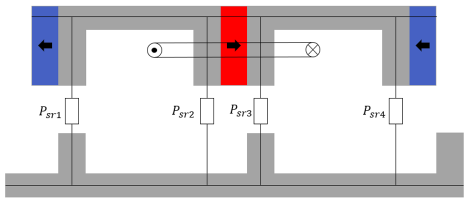
\includegraphics[scale=0.7]{Perm.png}
    \caption{2D linear model of an FSPM and corresponding permeance circuit}
\end{figure}
 Here we assume that the current and the magnetic flux are sinusoidal. We will express the total flux linkage $\Phi_{PM}$ as the product of the maximum flux linkage for a single coil $\phi_{a}$ times the number of turns per phase $N_{a}$.
 $$ T_{em} = \frac{3}{2}N_{r}\psi_{PM}I_{q} = \frac{3}{2}N_{r}N_{a}\phi_{a}I_{q}$$
 The maximum flux linkage $\phi_{a}$ can be determined with the structure of the FSPM. The maximum value is two times the flux generated by a magnet, $2\phi_{m}$. This flux can be expressed as the integral of the magnetic field produced by the magnet, we assume that this magnetic field is constant.
 
 $$ \phi_{m} = \int \int_{S} \overrightarrow{B} ~.~ \overrightarrow{dS} = B_{m}(R_{0}-R_{i})l_{a} $$
 
 There are three coefficient that will reduce the value of the maximal flux linkage which are the winding factor, $k_{w}$, the flux leakage factor, $\sigma_{0}$, and a geometrical factor, $k_{a}$. The winding factor will be assumed to be constant for now and is described further. The flux leakage factor correspond to the flux losses between the magnets and the coil and will also be assumed to be constant. The last one, $k_{a}$, is based on the permeance equivalent circuit. The equation for a stator tooth depends on the four permeance associated with it. 
 
 \begin{figure}[H]
    \centering
    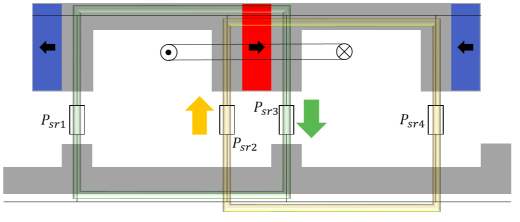
\includegraphics[scale=0.7]{ka.png}
    \caption{}
\end{figure}
 
 $$ N_{r}k_{a} = N_{r}(\frac{P_{sr3}}{P_{sr3}+P_{sr4}}-\frac{P_{sr2}}{P_{sr1}+P_{sr2}}) $$
 
 The permeance of a ferromagnetic tooth of the stator is maximized when the rotor tooth is aligned with it. In the configuration on the previous picture for example, $P_{sr1}$ and $P_{sr3}$ are maximum and $P_{sr2}$ and $P_{sr4}$ are minimum. It leads to $k_{a} \simeq 1$ and the opposite situation would lead to $k_{a} \simeq -1$.
 
 we can now look at the complete expression for the interaction between one single stator tooth and the complete rotor. The permeance with all harmonics can be expressed as : 
 
 $$ P_{sr}(\theta_{sr}) = P_{0} + \sum_{v=1,3,5,...} P_{v}cos(N_{r}v\theta_{sr})$$
 
 We will make some simplification in our model of the permeance. We will only consider the first harmonic, we supposed that the other ones are neglectable. We will suppose that $P_{0} \approx P_{1}$ what means that the permeance will be null if the rotor tooth and the ferromagnetic tooth at the stator are perfectly unaligned. And finally we will uniform the dimension to simplify the expressions.
 
  \begin{figure}[H]
    \centering
    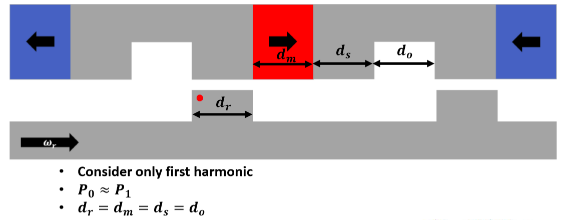
\includegraphics[scale=0.6]{simp.png}
    \caption{}
\end{figure}
 
 This leads to a simplified expression for the permeance ; 
 
 $$ P_{srk} = P_{sr}(\theta_{srk}) = P_{0} + P_{0} cos(N_{r}\theta_{0sr} + \frac{(5-2k)N_{r}\pi}{2N_{s}})$$
 
 With $\theta_{0sr}$ the relative angle between the stator and the rotor. 
 
 From this equation and the expression of $k_{a}$ we can deduce a relation between $k_{a}$ and the number of poles in the rotor and the stator. We take this at the maximum flux ($\theta_{0sr} = \pi / 2N_{r}$) and we get : 
 
 $$ k_{a} = \sum_{i=0}^{1} (-1)^{i} \frac{1+sin((-1)^{i}(N_{r}\pi/2N_{s}))}{2 + 2cos(N_{r}\pi/2N_{s})sin((-1)^{i}(N_{r}\pi/N_{s}))} $$
 
 At this point to maximize the torque we have to maximize $k_{a}$. We will look at the maximum in therms of number of poles at the rotor (here for example we take 12 stator poles). 
 
   \begin{figure}[H]
    \centering
    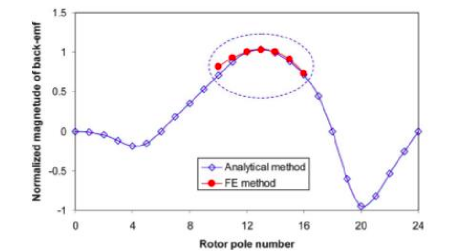
\includegraphics[scale=0.7]{max.png}
    \caption{}
\end{figure}
 
 We see that the maximum is obtained when we have the same number of poles at the stator and at the rotor. But we can't choose this solution because of the cogging torque and the preferential positioning that we want to avoid. We have three conditions on $N_{s}$ : it has to be even, a multiple of the number of phases, and different from $N_{r}$. Finally it gives : 
 
$$ N_{s} = k_{1}m ~~~~;~~~~ N_{r} = N_{s} \pm k_{2} $$
$$ k_{1} = 1,2,... ~~~~;~~~~ k_{2} = 1,2,... $$

With $m$ the number of phases and where $k_{1}$ is even if $m$ is odd.

In order to maximize the torque we will then take the number of poles at the rotor as close as possible as the number of poles at the stator but always different. The different possibilities are discussed further.

\section{Winding connection}
Now that we understand the operating principle of the FSPM machine, we will study how to connect the windings together to optimize its effect. The first objective of this connection is to group the windings and form the different phases, usually 3. Here is the relation between the mechanical degrees and the electrical degrees :

$$ \alpha_e = N_r * \alpha_m$$

where $N_r$ is the number of rotor poles. The mechanical degrees simply represent the positions of the stator coils and the electrical degrees refer to the phase shift of the back-EMF's. We can represent the coil position vectors and the associated back-EMF phasors :

\begin{figure}[H]
\centering
\begin{subfigure}{.5\textwidth}
  \centering
  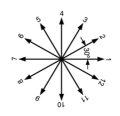
\includegraphics[scale = 0.5]{coils.png}
  \caption{Coils positions}
\end{subfigure}%
\begin{subfigure}{.5\textwidth}
  \centering
  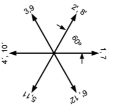
\includegraphics[scale = 0.5]{emf_phasors.png}
  \caption{Back-EMF phasors}
\end{subfigure}
\captionsetup{justification=centering}
\caption{Coils positions and back-EMF phasors for a 12/14 stator/rotor poles machine. As an example, coil 3 is at 60° from coil 1 so its associated back-EMF will have a phase shift of $14*60 = 2*360 + 120$ = 120°}
\end{figure}

The EMF phasors allow to visualize the voltages induced in the different windings.
As it can be seen in Figure 7 b), even phasors are noted with a ' while odd phasors not. This is because of the polarity of the magnet which is inside the coil. Two successive magnets are of opposite polarity, so this will imply a 180° phase shift on the back-EMF. Now we want to associate these EMF phasors in order to obtain a balanced 3-phase system. Each phase has thus to be shifted by $2\pi/3$ from one another. 

\begin{figure}
    \centering
    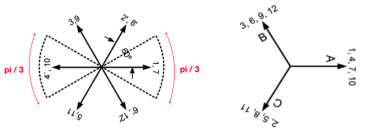
\includegraphics[scale=0.5]{3phase.png}
    \caption{Combination of EMF phasors to produce a 3-phase system}
\end{figure}

The phasor of each phase is the vectorial sum of the back-EMF phasors that will constitute the phase. Phasors with a ' are multiplied by -1 and then added to the other phasors. In this case, phase A consists of the sum of phasors 1, 4, 7 and 10 (as showed in Figure 8). That means that coils 1, 4, 7 and 10 are connected togheter. This is the only possible configuration for a 12/14 stator/rotor FSPM machine since it is the only one who maximizes the total EMF.

For a 12/13 stator/rotor machine, the methodology has to be adapted. We see that inside a single phase, there is a phase shift between the back-EMF phasors. We say that the windings are distributed. The winding factor has to be maximized as explained in the following section : we will see that the vectorial sum has to be maximized. To do this, we have to select the EMF phasors which are the closest from each other.

\begin{figure}
    \centering
    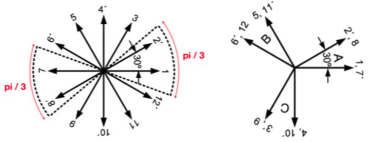
\includegraphics[scale = 0.5]{13poles.png}
    \caption{12/13 stator/rotor poles machine}
\end{figure}



\section{Winding factor}
The winding factor is the ratio between the flux that is actually intercepted and that could be intercepted by a coil if it was a single layer full pitch integer-slot winding with the same number of turns and one single slot per pole per phase. 
In this seminar it is defined as : 
\begin{equation}
    k_w = k_d k_p
\end{equation}
with $k_d$ the distribution factor and $k_p$ the pitch factor. 

\subsection{Distribution factor}
The distribution factor is due to the winding coils being distributed in a number of slots, and the induced EMF by each slot sums vectorially. The distribution factor is the ratio between this real vectorial sum and the ideal arithmetic sum. This is shown in Figure \ref{fig:distributionfactor}
\begin{figure}[H]
    \centering
    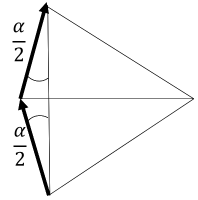
\includegraphics[width=0.25\textwidth]{distributionfactor.png}
    \caption{Distribution factor}
    \label{fig:distributionfactor}
\end{figure}
This is defined as : 
\begin{equation}
    k_d = \frac{\text{phasor sum of all EMF components}}{\text{arithmetic sum of all EMF components}} = \frac{sin \left ( \frac{\pi}{2mp}\right)}{\frac{s}{2mp} sin \left(\frac{\pi}{s}\right)}
\end{equation}

\subsection{Pitch factor}
The pitch factor is linked to the fact that the windings are often not fully pitched. The individual turns are reduced in order to decrease the length of the end turns and do not cover a full pitch. This is shown in Figure \ref{fig:pitchfactor}.
\begin{figure}[H]
    \centering
    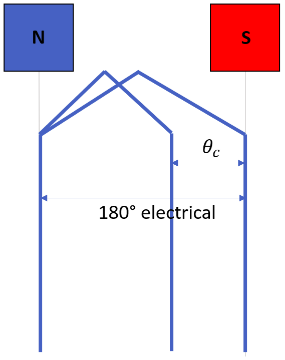
\includegraphics[width=0.25\textwidth]{pitchfactor.png}
    \caption{Pitch factor}
    \label{fig:pitchfactor}
\end{figure}
The mathematical definition is given by : 
\begin{equation}
    k_p = \frac{\text{EMF of short pitched coil}}{\text{EMF of full pitched coil}} = \frac{ \int_{\alpha/2}^{180-\alpha/2} sin (\theta) d\theta
    }{\int_{0}^{180} sin (\theta) d\theta
    } = cos(\alpha/2)
\end{equation}


\section{Back-Emf}
One of the problems with FSPM machines is that the flux linkage and the back-EMF waveforms of an individual winding are asymmetric and they may have asymmetrical back-emf force with certain number of pole combinations.\\
A half-wave symmetrical signal is a waveform whose first half-period is the opposite of the second half-period.
\begin{figure}[H]
    \centering
    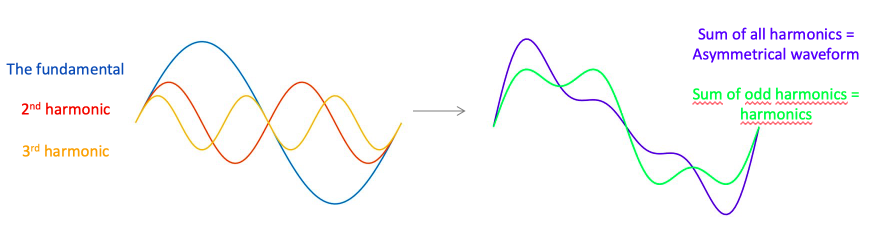
\includegraphics[scale=0.4]{symm.png}
    \caption{Symmetric and asymmetric waveforms}
\end{figure}
In order to obtain such a signal, the even harmonics have to be cancelled out. We do this by subtracting the same phase-shifted signal of $180\degree$. 

In fact, this is exactly what we did, in Section 3, when we brought opposite emf vectors back into the same phase.

In other words, the number of coils per phase should be even in order that the machine can be designed such that phase winding comprises one or more pairs of coils having a phase shift of 180 electrical degrees between the coils.%To have a counter-ectromotive symmetric force, it is necessary to be in a configuration where one has for each emf vector its opposite in the same phase.

This condition can be rewritten as an equation.\footnote{This part was not presented during the seminar and was not deemed essential by the professor but is nevertheless explained in this section.} The equation is as follows: $$\frac{2\pi \cdot N_r \cdot n_{pp}}{N_s} = (2k-1)\pi$$
with $n_{pp}$ as the number of poles between two emf of the same phase and therefor $2\pi N_r n_{pp}/N_s$ being the electric angular difference between two coils in an one phase and k an integer.

This expression becomes\footnote{The demonstration required to arrive to this expression is complicated and not interesting.}: $$\frac{N_s}{HCF(N_s , N_r)}=\text{even number}$$
where HCF is the highest common factor (=PGCD : plus grand commun diviseur).\\
Depending on the different cases described in Section 3, we have different constraints: (where j is an integer)

\begin{minipage}[b]{0.22\linewidth}
\textbf{\small{All-poles m is odd}}
\end{minipage}
\hspace{0.2cm}
\begin{minipage}[b]{0.22\linewidth}
\textbf{\small{All-poles m is even}}
\end{minipage}
\hspace{0.35cm}
\begin{minipage}[b]{0.22\linewidth}
\textbf{\small{Alter-poles m is odd}}
\end{minipage}
\hspace{0.3cm}
\begin{minipage}[b]{0.22\linewidth}
\textbf{\small{Alter-poles m is even}}
\end{minipage}

\begin{minipage}[b]{0.2\linewidth}
\begin{center}
$\frac{N_s}{HCF(N_s , N_r)}=2jm$    
\end{center}
\end{minipage}
\hspace{0.4cm}
\begin{minipage}[b]{0.22\linewidth}
\begin{center}
$\frac{N_s/2}{HCF(N_s/2 , N_r/2)}=jm$
\end{center}
\end{minipage}
\hspace{0.4cm}
\begin{minipage}[b]{0.22\linewidth}
\begin{center}
$\frac{N_s}{HCF(N_s , N_r)}=2jm$
\end{center}
\end{minipage}
\hspace{0.4cm}
\begin{minipage}[b]{0.22\linewidth}
\begin{center}
$\frac{N_s/2}{HCF(N_s/2 , N_r/2)}=jm$
\end{center}
\end{minipage}

We apply and observe the conditions for the back-EMF symmetry theory with  the equations above for different stator/rotor combinations:
%The example here is a machine, with 12/13 poles stator / rotor all poles wound. We see on the right that as soon as we are the coils 1 and 7 '(which are opposed), the harmonic of order 2 is the trunk.In the following figure (machine ALTErNATE poles wound, Ns = 12), we see what happens when the relationship is not respected (Ns = 12 and Nr = 10 or 14): it's not symmetrical, and so it's ugly.

\begin{minipage}[b]{0.46\linewidth}
    \begin{figure}[H]
        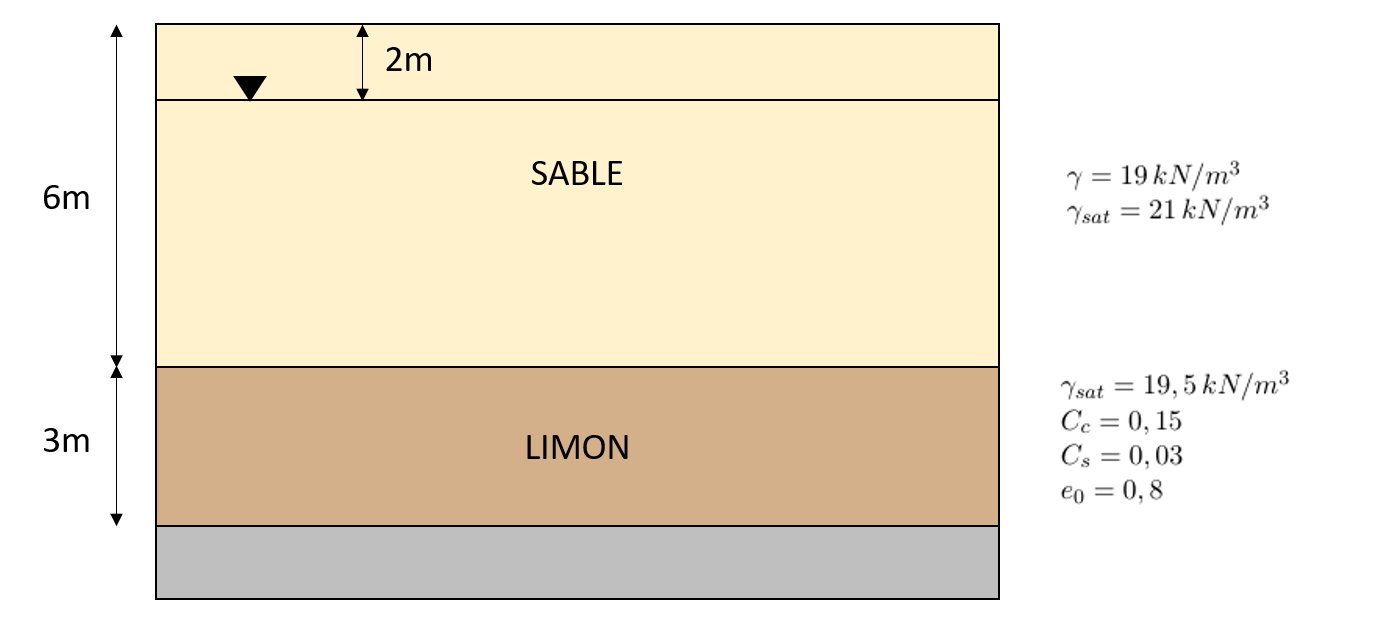
\includegraphics[scale=0.45]{ex1.png}
        \caption{Back-EMF of 12/13 stator/rotor machine. \\(a) Waveforms. (b) Spectra.}
    \end{figure}
\end{minipage}
\begin{minipage}[b]{0.46\linewidth}
\begin{itemize}
    \item Back-EMF waveforms of coils 1, 7’ , 2’ and 8 are asymmetrical. (harmonic 2)
    \item The resultant waveforms (1 - 7, 2’- 8’ and 1 - 7 + 2’- 8’) are symmetrical. (harmonics 2 cancelled)
    \item Not purely sinusoidal. (harmonic 5)
\end{itemize}
\end{minipage}

\begin{minipage}[b]{0.46\linewidth}
\begin{itemize}
    \item Back-EMF waveforms of coils 1, 4 , 7 and 10 are asymmetrical. (harmonics 2 and 6)
    \item Waveform (1+7+4+10) is symmetrical. (harmonics 2 and 6 cancelled)
    \item Not purely sinusoidal. (harmonic 6)
\end{itemize}
\end{minipage}
\begin{minipage}[b]{0.46\linewidth}
    \begin{figure}[H]
    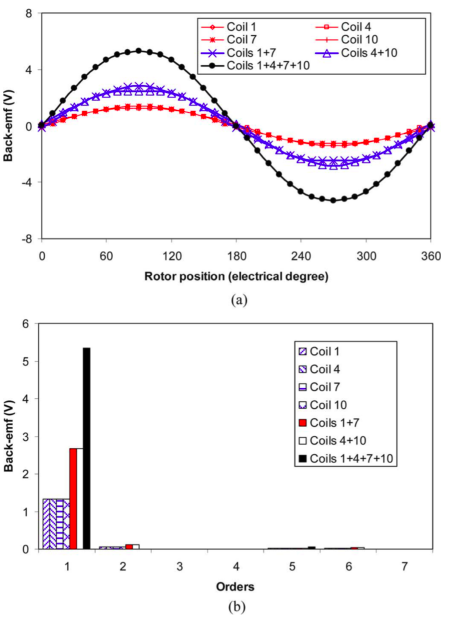
\includegraphics[scale=0.45]{ex2.png}
    \caption{Back-EMF of 12/14 stator/rotor machine.\\ (a) Waveforms. (b) Spectra.}
    \end{figure}
\end{minipage}


\section{Unbalanced Magnetic Force (UMF)}
UMF can be computed based on the Maxwell stress tensor : 
\begin{equation}
    \sigma_{M,ij} = 
    \epsilon_0 \left( E_i E_j - \frac{1}{2}\delta_{ij}E^2\right)
    -\frac{1}{\mu_0}\left( B_i B_j -\frac{1}{2}\delta_{ij}B^2\right)
\end{equation}
With : 
\begin{itemize}
    \item $\sigma_{M,ij}$ the components of the Maxwell stress tensor
    \item $E$ the electric field 
    \item $B$ the magnetic field
\end{itemize}

Knowing that we only consider contribution of the magnetic field, we can construct the matrix as shown in Figure \ref{fig:maxwellst}
\begin{figure}[H]
    \centering
    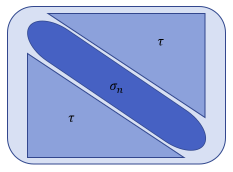
\includegraphics[width=0.3\textwidth]{MaxwellST.png}
    \caption{Maxwell stress tensor, components type}
    \label{fig:maxwellst}
\end{figure}
With : $\sigma_n = \frac{B_r^2 = B_\alpha^2}{2\mu_0}$ and $\tau= \frac{B_rB_\alpha}{\mu_0}$
The components are then project on x- and y-axis and integrated leading to x- and y-components of the UMF. These components can be decomposed in a sum of a radial term due to $\sigma_n$ and a tangential term due to $\tau$. As the tangential term just interacts with the torque, we will only focus on the impacts of the radial component that we name 'resultant UMF'. 
\begin{equation}
    F_{rx} = \frac{rl_a}{2\mu_0} \int_0^{2\pi} (B_\alpha^2 - B_r^2) cos \alpha d\alpha\\
    F_{ry} = \frac{rl_a}{2\mu_0} \int_0^{2\pi} (B_\alpha^2 - B_r^2) sin \alpha d\alpha
\end{equation}

The effects of UMF on the machine are unwanted constraints and vibrations which can result in noise and even damages to the machine. The solution to avoid these effects is to have an UMF as small and constant as possible around the axis, avoiding pulsations. This can be obtained by increasing the numbers of poles. In the graphs presented in Figures \ref{fig:umf65}, \ref{fig:umf67}, \ref{fig:umf1211} and \ref{fig:umf1213}, it can be seen that 6/5 and 6/7 poles machines show strongly pulsative UMF, with a far bigger amplitude than 12/11 and 12/13 poles machines. It also shows that having all or alternates poles does not make a crucial difference for radial UMF. 
\begin{figure}
    \centering
    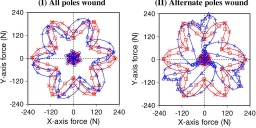
\includegraphics[width = 0.4\textwidth]{UMF65.png}
    \caption{UMF 6/5 all and alternate poles wound}
    \label{fig:umf65}
    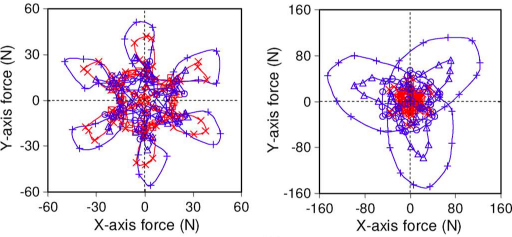
\includegraphics[width = 0.4\textwidth]{UMF67.png}
    \caption{UMF 6/7 all and alternate poles wound}
    \label{fig:umf67}
    \centering
    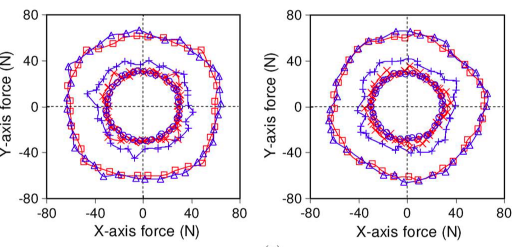
\includegraphics[width = 0.4\textwidth]{UMF1211.png}
    \caption{UMF 12/11 all and alternate poles wound}
    \label{fig:umf1211}
    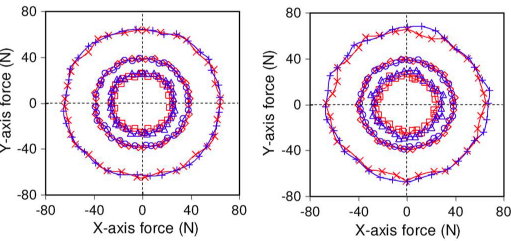
\includegraphics[width = 0.4\textwidth]{UMF1213.png}
    \caption{UMF 12/13 all and alternate poles wound}
    \label{fig:umf1213}
\end{figure}
